\begingroup
\hyphenpenalty=10000\exhyphenpenalty=10000
\definecolor{IEEEBlue}{HTML}{00629B}
\definecolor{Cyan}{HTML}{00A6B2}
\definecolor{Navy}{HTML}{003B5C}
\definecolor{Slate}{HTML}{526470}
\definecolor{RestRed}{HTML}{B83136}
\definecolor{RestAmber}{HTML}{A66610}
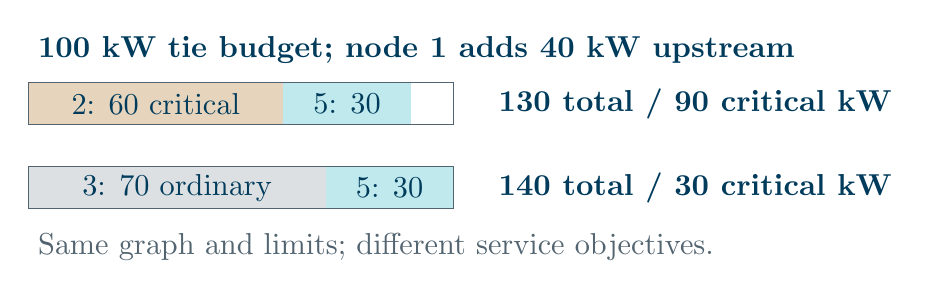
\begin{tikzpicture}[x=.90cm,y=.82cm,font=\fontsize{11}{12}\selectfont,
  every node/.style={text=Navy},
  flow/.style={-{Stealth[length=2mm]},line width=1pt,draw=IEEEBlue},
  bus/.style={circle,draw=IEEEBlue,line width=1pt,minimum size=5.5mm,inner sep=1pt,fill=white},
  textblock/.style={align=center,inner sep=1pt},
  pass/.style={draw=Cyan,line width=2pt},
  available/.style={draw=Slate,line width=.8pt},
  optional/.style={draw=RestAmber,dashed,line width=1pt}]

\node[anchor=west] at (0,3.1) {\textbf{100 kW tie budget; node 1 adds 40 kW upstream}};
\fill[RestAmber!28] (0,1.95) rectangle (3.6,2.6);
\fill[Cyan!25] (3.6,1.95) rectangle (5.4,2.6);
\draw[Slate] (0,1.95) rectangle (6,2.6);
\node at (1.8,2.27) {2: 60 critical};
\node at (4.5,2.27) {5: 30};
\node[anchor=west] at (6.5,2.27) {\textbf{130 total / 90 critical kW}};
\fill[Slate!20] (0,.65) rectangle (4.2,1.3);
\fill[Cyan!25] (4.2,.65) rectangle (6,1.3);
\draw[Slate] (0,.65) rectangle (6,1.3);
\node at (2.1,.97) {3: 70 ordinary};
\node at (5.1,.97) {5: 30};
\node[anchor=west] at (6.5,.97) {\textbf{140 total / 30 critical kW}};
\node[anchor=west,text=Slate] at (0,.05) {Same graph and limits; different service objectives.};

\end{tikzpicture}
\endgroup
